\documentclass{jfp1}

%%%%%%%%%%%%%%%%%%%%%%%%%%%%%%%%%%%%%%%%%%%%%%%%%%%%%%%%%%%%
% Global switches
%%%%%%%%%%%%%%%%%%%%%%%%%%%%%%%%%%%%%%%%%%%%%%%%%%%%%%%%%%%%

% Turn on to include todos and comments.  These are intended for stuff
% we need to do or discussions that may influence the text of the
% paper itself.
\newif\ifcomments\commentstrue

% Turn on to include commentary. This is intended for stuff we want to
% remember/write down but do not intend to include in the paper.
\newif\ifcommentary\commentarytrue

%%%%%%%%%%%%%%%%%%%%%%%%%%%%%%%%%%%%%%%%%%%%%%%%%%%%%%%%%%%%
% Packages
%%%%%%%%%%%%%%%%%%%%%%%%%%%%%%%%%%%%%%%%%%%%%%%%%%%%%%%%%%%%

\usepackage[T1]{fontenc}
\usepackage[utf8]{inputenc}
\usepackage[override]{cmtt}
\usepackage{hyperref}
\usepackage{mdframed}
\usepackage{comment}

\usepackage{graphicx}
\graphicspath{{images/}}

\usepackage{latex/agda}
% for grabbing pieces of Agda from a different file, so that latex and
% Agda don't have to mix too much.
\usepackage{catchfilebetweentags}

\usepackage[backend=pgf, outputdir=diagrams]{diagrams-latex}

%%%%%%%%%%%%%%%%%%%%%%%%%%%%%%%%%%%%%%%%%%%%%%%%%%%%%%%%%%%%
% Unicode
%%%%%%%%%%%%%%%%%%%%%%%%%%%%%%%%%%%%%%%%%%%%%%%%%%%%%%%%%%%%

% See https://agda.readthedocs.io/en/v2.6.0.1/tools/generating-latex.html

\usepackage{newunicodechar}
\newunicodechar{∀}{\ensuremath{\forall}}
\newunicodechar{ℓ}{\ensuremath{\ell}}
\newunicodechar{→}{\ensuremath{\to}}
\newunicodechar{λ}{\ensuremath{\lambda}}
\newunicodechar{ℕ}{\ensuremath{\mathbb{N}}}
\newunicodechar{∘}{\ensuremath{\circ}}

%%%%%%%%%%%%%%%%%%%%%%%%%%%%%%%%%%%%%%%%%%%%%%%%%%%%%%%%%%%%
% Typesetting
%%%%%%%%%%%%%%%%%%%%%%%%%%%%%%%%%%%%%%%%%%%%%%%%%%%%%%%%%%%%

\newcommand{\term}[1]{\emph{#1}}

%%%%%%%%%%%%%%%%%%%%%%%%%%%%%%%%%%%%%%%%%%%%%%%%%%%%%%%%%%%%
%% Comments
%%%%%%%%%%%%%%%%%%%%%%%%%%%%%%%%%%%%%%%%%%%%%%%%%%%%%%%%%%%%

\ifcomments
\newcommand{\authornote}[3]{\textcolor{#1}{[#3 ---#2]}}
\newcommand{\todo}[1]{\textcolor{red}{[TODO: #1]}}
\else
\newcommand{\authornote}[3]{}
\newcommand{\todo}[1]{}
\fi

\newcommand{\bay}[1]{\authornote{blue}{BAY}{#1}}
\newcommand{\jc}[1]{\authornote{green}{JC}{#1}}  % pick whatever
                                                 % color/initials you want

\ifcommentary
  \newmdenv[skipabove=1em, skipbelow=1em, innermargin=1.5em, outermargin=1.5em, backgroundcolor=black!8, linecolor=black!10]{commentary}
\else
  \excludecomment{commentary}
\fi

%%%%%%%%%%%%%%%%%%%%%%%%%%%%%%%%%%%%%%%%%%%%%%%%%%%%%%%%%%%%
% Front matter
%%%%%%%%%%%%%%%%%%%%%%%%%%%%%%%%%%%%%%%%%%%%%%%%%%%%%%%%%%%%

\title{Memory Models via Species: The Paper}
\subtitle{Or: You Could Have Invented Species, If You Happened To Think
  About It In This Very Specific Way}
\author[J. Carette and B. A. Yorgey]{JACQUES CARETTE\\
  McMaster University, Ontario, Canada \\
  \email{carette@mcmaster.ca}
  \and BRENT A. YORGEY\\
  Hendrix College, Arkansas, USA\\
  \email{yorgey@hendrix.edu}}

%%%%%%%%%%%%%%%%%%%%%%%%%%%%%%%%%%%%%%%%%%%%%%%%%%%%%%%%%%%%

\begin{document}

\maketitle

What is a \term{memory}?  We will start by taking the abstract
position that \emph{a memory is a store of values}, that is, a place
where values can be stored and later retrieved.

\begin{figure}[htp]
  \centering
  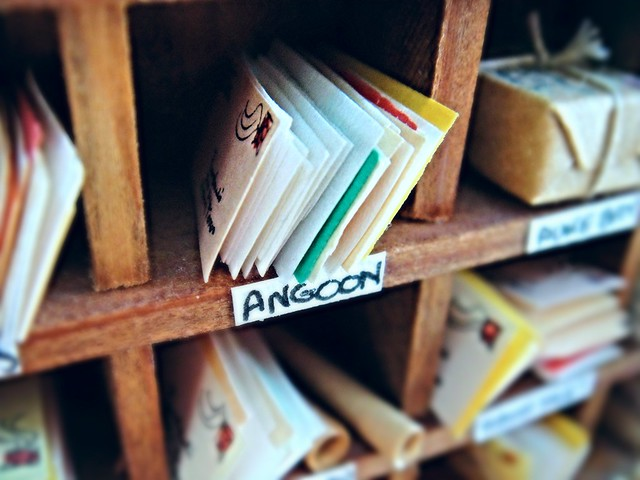
\includegraphics[width=0.5\textwidth]{mailboxes.jpg}
  \caption{A memory with labelled locations. Photo by JLS Photography.\protect\footnotemark}
  \label{fig:mailboxes}
\end{figure}
\footnotetext{\url{https://www.flickr.com/photos/akgypsy37/8690531067/}, CC BY-NC-ND 2.0.}

What sort of structure does a memory need to have to make this
possible?  In order to be able to retrieve values after storing them,
there must be some way to refer to values by their location, so we
suppose that each location has a \emph{label}.  Then a \term{memory}
is just a mapping from labels to values.

\ExecuteMetaData[latex/models.tex]{memory}

For now, we don't assume that labels have any additional structure,
though some particular sets of labels might.  For example, the
locations in Figure~\ref{fig:mailboxes} are evidently arranged in a 2D
grid, but this is special.  In the abstract, it may be helpful to
imagine a memory as a ``soup'' of locations.

\todo{Diagram the soup.}

\todo{Go deeper into the soup: We're going to use Agda as our
  metalogic, but no commitments to the metalogic.  E.g. no assumptions
  about whether label/value types can be represented/constructed,
  i.e. whether they actually exist at runtime. Don't assume we can do
  sums, products, etc. on types}

\begin{commentary}
  Labels could be real numbers.  But we won't be able to do much with
  that.  We quickly want decidable equality for labels.

  Models with and without functoriality for values!  Might have to do
  something like co-Yoneda trick to make it functorial.
\end{commentary}

\todo{motivate relabel: one model is to actually change the labels.
  Another is to just store a function off to the side.  e.g. array
  libraries, virtual memory}

\ExecuteMetaData[latex/models.tex]{relabel}

\todo{draw a picture of relabelling.}

Note that a $\AgdaFunction{Memory}$ must be a \emph{total} function,
that is, every label corresponds to some value.  If we wish to model
memories where some labels do not correspond to a stored value, we can
simply use a type $V$ of values with a distinguished ``empty'' value.
\todo{Actually there are other choices too!  e.g. get rid of labels
  entirely.  This is why we're going to wait.}

Alternatively,

\begin{commentary}
  relabel is still useful if $L' = L$.  e.g. Copying garbage collection.
\end{commentary}

\todo{eventual motivation: represent data structures!  So we need some
structure on labels (?)  Next up: disjoint union.  Related to malloc:
what to do if someone hands you some new labels.  Look at haskell/src/Data/Storage.hs}


\end{document}
